%%%%%%%%%%%%%%%%%%%%%%%%%%%%%%%%%%%%%%%%%%%%%%%%%%%%%%%%%%%%%%%%%%%%%%%%%%%%%%%%%%%%
% Document data
%%%%%%%%%%%%%%%%%%%%%%%%%%%%%%%%%%%%%%%%%%%%%%%%%%%%%%%%%%%%%%%%%%%%%%%%%%%%%%%%%%%%
\documentclass[12pt]{article} %report allows for chapters
%%%%%%%%%%%%%%%%%%%%%%%%%%%%%%%%%%%%%%%%%%%%%%%%%%%%%%%%%%%%%%%%%%%%%%%%%%%%%%%%%%%%
\usepackage{preamble}
\newcommand{\grad}{\boldsymbol{\vec{\nabla}}}
\newcommand{\curvegamma}{\boldsymbol{\vec{\gamma}}}
\newcommand{\tangentgamma}{\boldsymbol{\dot{\vec{\gamma}}}}
\newcommand{\normalgamma}{\boldsymbol{\ddot{\vec{\gamma}}}}
\newcommand{\vecfieldE}{\boldsymbol{\vec{E}}}
\newcommand{\rhat}{\boldsymbol{\hat{r}}}
\newcommand{\thetahat}{\boldsymbol{\hat{\theta}}}
\newcommand{\phihat}{\boldsymbol{\hat{\phi}}}
\newcommand{\rhohat}{\boldsymbol{\hat{\rho}}}
\newcommand{\unitvec}{\boldsymbol{\hat{n}}}
\newcommand{\vecfieldB}{\boldsymbol{\vec{B}}}
\newcommand{\vecfieldJ}{\boldsymbol{\vec{J}}}
\newcommand{\vecfieldF}{\boldsymbol{\vec{F}}}
\newcommand{\vecfieldV}{\boldsymbol{\vec{V}}}
\newcommand{\vecfieldU}{\boldsymbol{\vec{U}}}
\newcommand{\vf}[1]{\boldsymbol{\vec{#1}}}

\begin{document}

\begin{center}
   \textsc{\large MATH 272, Homework 3. \emph{Solutions}.}\\
\end{center}
\vspace{.5cm}





%\newpage
%\begin{problem}
%Consider the two dimensional scalar field $T(x,y)=x+y$ that describes the temperature on the square plate $\Omega$ given by the set $0\leq x,y \leq 1$.  Compare the two answers you get!
%\begin{enumerate}[(a)]
%	\item Compute the integral
%	\[
%	\int_\Omega T d\Omega.
%	\]
%	\item Let $\curvegamma$ be the curve that traverses the boundary of the square plate in the counterclockwise direction.  Compute
%	\[
%	\int_{\curvegamma} T d\curvegamma. 
%	\]
%\end{enumerate}
%\end{problem}
%\begin{solution} ~
%	\begin{enumerate}[(a)]
%		\item We take
%		\begin{align*}
%			\iint_\Omega T(x,y)d\Omega &= \int_0^1 \int_0^1 x+y dxdy\\
%			&= \int_0^1 \left.\left(\frac{1}{2}x^2+xy\right)\right\vert_0^1 dy\\
%			&= \int_0^1 \frac{1}{2} + y dy\\
%			&= \left.\left(\frac{1}{2}y + \frac{1}{2}y^2\right)\right\vert_0^1\\
%			&= 1.
%		\end{align*}
%		\item	First, note that there are four straight curves that parameterize the boundary of the plate.  Namely, we can choose the parameterizations 
%		\[
%		\curvegamma_1(t) = \begin{pmatrix} t \\ 0 \end{pmatrix} \quad \curvegamma_2(t) = \begin{pmatrix} 1 \\ t \end{pmatrix} \quad \curvegamma_1(t) = \begin{pmatrix} 1-t \\ 1 \end{pmatrix} \quad \curvegamma_1(t) = \begin{pmatrix} 0 \\ 1-t \end{pmatrix},
%		\]
%		Note that there are many other parameterizations that work. We can see the chosen curves in this figure:
%		\begin{figure}[H]
%			\centering
%			\includegraphics[width=.6\textwidth]{figures/plate_boundary.png}
%		\end{figure}
%		Thus, our integral can be written as
%		\[
%		\int_{\curvegamma} T(\curvegamma) d\curvegamma = \int_{\curvegamma_1} T(\curvegamma) d\curvegamma_1 + \int_{\curvegamma_2} T(\curvegamma) d\curvegamma_2 + \int_{\curvegamma_3} T(\curvegamma) d\curvegamma_3 + \int_{\curvegamma_4} T(\curvegamma) d\curvegamma_4.
%		\]
%		Then, we can compute each integral on the right hand side.
%		\begin{align*}
%			\int_{\curvegamma_1} T(\curvegamma_1) d\curvegamma_1 &= \int_0^1 T(\curvegamma_1(t))\left|\tangentgamma_1(t)\right|dt\\
%			&= \int_0^1 T(t,0) dt\\
%			&= \int_0^1 t dt\\
%			&= 1.
%		\end{align*}
%		Similarly, 
%		\begin{align*}
%				\int_{\curvegamma_2} T(\curvegamma_2) d\curvegamma_2 &= \int_0^1 T(\curvegamma_2(t))\left|\tangentgamma_2(t)\right|dt\\
%				&= \int_0^1 T(1,t) dt\\
%				&= \int_0^1 1+t dt\\
%				&= \left.\left(t+\frac{1}{2}t^2\right)\right\vert_0^1\\
%				&= \frac{3}{2}.
%		\end{align*}	
%		Again,
%		\begin{align*}
%				\int_{\curvegamma_3} T(\curvegamma_3) d\curvegamma_3 &= \int_0^1 T(\curvegamma_3(t))\left|\tangentgamma_3(t)\right|dt\\
%				&= \int_0^1 T(1-t,1) dt\\
%				&= \int_0^1 (1-t)+1 dt\\
%				&= \int_0^1 2-tdt\\
%				&= \left.\left( 2t-\frac{1}{2}t^2\right)\right\vert_0^1\\
%				&= \frac{3}{2}.
%		\end{align*}			
%		Lastly,
%		\begin{align*}
%			\int_{\curvegamma_4} T(\curvegamma_4) d\curvegamma_4 &= \int_0^1 T(\curvegamma_4(t))\left|\tangentgamma_4(t)\right|dt\\
%			&= \int_0^1 T(0,1-t) dt\\
%			&= \int_0^1 1-t dt\\
%			&= \left.\left(t-\frac{1}{2}t^2\right)\right\vert_0^1\\
%			&= \frac{1}{2}.
%		\end{align*}	
%	\end{enumerate}
%	Thus, we have
%	\[
%	\boxed{\int_{\curvegamma} T(\curvegamma) d\curvegamma = 1+\frac{3}{2}+\frac{3}{2}+\frac{1}{2} = \frac{9}{2}.}
%	\]
%\end{solution}

\begin{problem}
	\textbf{(6 pts.)} Parameterize the following either implicitly or explicitly. In Cartesian coordinates, find the parameterization of the normal vector as well.
	\begin{enumerate}[(a)]
		\item \textbf{(2 pts.)} The plane perpendicular to the vector $\vecv = \xhat + \yhat + \zhat$ passing through the point $(1,1,1)$.
		\item \textbf{(2 pts.)} The upper half of the unit disk in the $xy$-plane.
		\item \textbf{(2 pts.)} The surface of the unit sphere in $\R^3$.
	\end{enumerate}
\end{problem}
\begin{solution}~
\begin{enumerate}[(a)]
    \item The equation for a plane passing through a point $(x_0,y_0,z_0)$ perpendicular to a vector $\begin{pmatrix} a \\ b \\ c \end{pmatrix}$ is given by the implicit equation
    \[
    a(x-x_0)+b(y-y_0) + c(z-z_0) = 0.
    \]
    We are given the vector $\vecv = \begin{pmatrix} 1 \\ 1 \\ 1 \end{pmatrix}$ and $x_0=1$, $y_0=1$, and $z_0=1$ so we arrive at
    \[ 
    (x-1)+(y-1)+(z-1)=0.
    \]
    We plot this here.
    \begin{figure}[H]
        \centering
        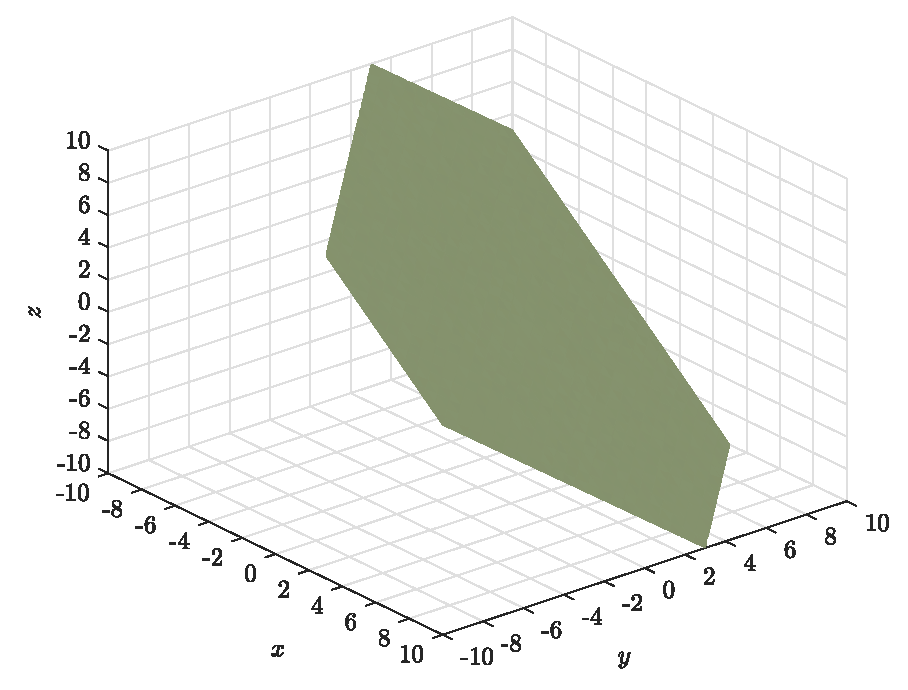
\includegraphics[width=.6\textwidth]{figures/plane}
        \caption{A plot of the plane satisfying our restrictions. Note the plane extends infinitely, but it is cropped by the axes in Matlab.}
    \end{figure}
    The normal vector is constant on a plane and is already being described via $\vecv$. To get the normal vector, we simply normalize $\vecv$ and we find
    \[
    \unitvec = \frac{\vecv}{|\vecv|} = \frac{1}{\sqrt{3}} \begin{pmatrix} 1 \\ 1 \\ 1 \end{pmatrix}.
    \]
    It should be noted that flat surfaces will have constant normals!

    \item Since we are trying to determine a parameterization of the upper half of the unit disk in the $xy$-plane, we may first try to describe bits and pieces of this first. Namely, we have an equation for the unit circle in the $xy$-plane given by the equation
    \[
    x^2+y^2 = 1.
    \]
    Let's think about what this equation is saying a bit. Recall that the distance from the origin $\zerovec$ to the point $(x,y)$ in the $xy$-plane is $\sqrt{x^2+y^2}$ by the Pythagorean theorem. So, this equation is asking for all the points exactly a distance 1 away from the origin. Thus, if we wish to include the interior points, these are just the points that have a distance less than or equal to 1 from the origin. Hence, we should take
    \[
    x^2+y^2\leq 1,
    \]
    which we can graph.
    \begin{figure}[H]
        \centering
        \includegraphics[width=.6\textwidth]{figures/disk.png}
        \caption{Shaded region is the unit disk described by $x^2+y^2\leq 1$.}
    \end{figure}
    Now, if we want just the upper half of this disk, we must require $y\geq 0$, as we can see in the next figure.
    \begin{figure}[H]
        \centering
        \includegraphics[width=.6\textwidth]{figures/disk_2.png}
        \caption{Red shade region is the unit disk described by $x^2+y^2\leq 1$ and the added constraint $y\geq 0$ is given in blue.}
    \end{figure}
    The overlap of the two colored regions gives us our domain of interest. The last requirement is that we also choose $z=0$. Thus, our parameterization is summarized as
    \begin{align*}
    x^2+y^2 &\leq 1 \\
    y &\geq 0\\
    z &= 0.
    \end{align*}
    Since this is a flat surface in the plane, the normal direction is the $\zhat$ direction. Hence, the surface normal can be chosen to be $\unitvec = \zhat$.
    
    \item We can follow our intuition from the previous part a bit. The surface of the unit sphere is the set of all points in $\R^3$ a distance of 1 away from the origin. The distance from the origin to a point $(x,y,z)$ is $\sqrt{x^2+y^2+z^2}$ again by the Pythagorean theorem. Hence, we have the implicit description
    \[
    \sqrt{x^2+y^2+z^2}=1,
    \]
    for which we could equivalently write
    \[
    x^2+y^2+z^2 =1.
    \]
    One can see previous homeworks for plots of this implicit surface.

    The normal to an implicit surface is $f(x,y,z)=0$ is
    \[
    \unitvec = \frac{\grad f}{|\grad f|},
    \]
    and in our case we have the function
    \[
    f(x,y,z) = x^2+y^2+z^2 -1 = 0.
    \]
    Then, 
    \[
    \grad f = \begin{pmatrix} 2x \\ 2y \\ 2z \end{pmatrix}
    \]
    for which we have
    \[
    |\grad f| = 2\sqrt{x^2+y^2+z^2}.
    \]
    Thus,
    \[
    \unitvec= \frac{x}{\sqrt{x^2+y^2+z^2}} \xhat  + \frac{y}{\sqrt{x^2+y^2+z^2}} \yhat  + \frac{z}{\sqrt{x^2+y^2+z^2}} \zhat.
    \]
\end{enumerate}
\end{solution}
\vspace*{1cm}
\textcolor{red}{
\noindent \textbf{Rubric:}
\begin{enumerate}[(a)]
    \item \textbf{(1 pt.)} Correct parameterization of the plane. \textbf{(1 pt.)} Correct normal vector.
    \item \textbf{(1 pt.)} Correct parameterization of the plane. \textbf{(1 pt.)} Correct normal vector.
    \item \textbf{(1 pt.)} Correct parameterization of the plane. \textbf{(1 pt.)} Correct normal vector.
\end{enumerate}
}

\newpage
\begin{problem}
\textbf{(5 pts.)} Consider $f(x,y)= 3x^4+x^3-18x^2y^2-3xy^2+3y^4$.
\begin{enumerate}[(a)]
    \item \textbf{(2 pts.)} Show $\Delta f = 0$.
    \item \textbf{(3 pts.)} Find the surface normal to the graph of $f$.
\end{enumerate}
\end{problem}
\begin{solution}~
\begin{enumerate}[(a)]
    \item We have
    \[
    \frac{\partial^2 f}{\partial x^2} = 6(6x^2+x-6y^2),
    \]
    which was computed using WolframAlpha by inputting:
    \begin{verbatim}
    D[3x^4+x^3-18x^2y^2-3xy^2+3y^4, {x,2}]
    \end{verbatim}
    Likewise,
    \[
    \frac{\partial^2 f}{\partial y^2} = -6(6x^2+x-6y^2),
    \]
    which again was computed via WolframAlpha by:
    \begin{verbatim}
    D[3x^4+x^3-18x^2y^2-3xy^2+3y^4, {y,2}]
    \end{verbatim}
    Thus,
    \[
    \Delta f = \frac{\partial^2 f}{\partial x^2} + \frac{\partial^2 f}{\partial y^2} = 0.
    \]
    \emph{Note: you can actually create a polynomial $f$ satisfying $\Delta f = 0$ (i.e., it is harmonic) by taking the real or imaginary part of any complex polynomial in the variable $z=x+iy$. This is how I created this!}

    \item We have the equation to the normal of a graph of $f(x,y)$ given by
    \[
        \unitvec = \frac{1}{\sqrt{1+\left(\frac{\partial f}{\partial x}\right)^2 + \left(\frac{\partial f}{\partial y}\right)^2}} \begin{pmatrix} -\frac{\partial f}{\partial x} \\ -\frac{\partial f}{\partial y} \\ 1 \end{pmatrix}.
    \]
    We have
    \[
    \frac{\partial f}{\partial x} = 3(4x^3+x^2-12xy^2-y^2) \qquad \textrm{and} \qquad \frac{\partial f}{\partial y} = -6y(6x^2+x-2y^2).
    \]
    Thus
    \[
    \boxed{\unitvec = \frac{1}{\sqrt{1 + \left( 3(4x^3+x^2-12xy^2-y^2) \right)^2 + \left( -6y(6x^2+x-2y^2) \right)^2 }} \begin{pmatrix} -3(4x^3+x^2-12xy^2-y^2) \\ 6y(6x^2+x-2y^2) \\ 1 \end{pmatrix}.}
    \]
    No real need to simplify further unless we are asked to.
\end{enumerate}
\end{solution}
\vspace*{1cm}
\textcolor{red}{
\noindent \textbf{Rubric:}
\begin{enumerate}[(a)]
    \item \textbf{(1 pt.)} Correct partial derivatives and work (or reference to WolframAlpha). \textbf{(1 pt.)} Correctly summed together to show you get zero.
    \item \textbf{(1 pt.)} Correct direction. \textbf{(1 pt.)} Correct normalization. \textbf{(1 pt.)} Correct final answer.
\end{enumerate}
}



\newpage
\begin{problem}
\textbf{(7 pts.)} Consider the following vector field
\[
\vecfieldE(x,y,z) = \begin{pmatrix} \frac{x}{(x^2+y^2+z^2)^{3/2}} \\ \frac{y}{(x^2+y^2+z^2)^{3/2}} \\ \frac{z}{(x^2+y^2+z^2)^{3/2}} \end{pmatrix},
\]
which models the electric field of a proton (in units of of charge $q=1$) placed at the origin. \emph{We have seen this before and will see it again later.}
\begin{enumerate}[(a)]
	\item \textbf{(1 pts.)} Show that $\vecfieldE(x,y,z) = - \grad \phi(x,y,z)$ where $\phi(x,y,z) = \frac{1}{\sqrt{x^2+y^2+z^2}}$.  We refer to $\phi(x,y,z)$ as the electrostatic potential (or voltage).
	\item \textbf{(4 pts.)} Let $\Omega$ be a box with side lengths two centered at the origin.  Compute the total flux of $\vecfieldE$ through the surface of the box $\Sigma$. That is,
	\[
	\int_\Sigma \vecfieldE \cdot \unitvec d\Sigma.
	\]
	\item \textbf{(2 pts.)} Using the provided argument, one can compute
	\[
	\int_\Omega \grad \cdot \vecfieldE d\Omega.
	\]
	\begin{itemize}
		\item Compute $\grad \cdot \vecfieldE$ and note that this is zero everywhere except at $(x,y,z)=(0,0,0)$. \emph{Hint: have you already done this?}
		\item Note that the two integrals in this problem are equal. This is known as the \emph{divergence theorem} and it is a special case of a more general theorem called \emph{Stokes' theorem} which generalizes the fundamental theorem of calculus. Is it true that $\grad \cdot \vecfieldE = 0$ everywhere?
	\end{itemize}
\end{enumerate}
\end{problem}
\begin{solution}~
    \begin{enumerate}[(a)]
        \item   We compute $-\grad \phi$,
        \begin{align*}
            -\grad \phi &= \begin{pmatrix} -\frac{\partial V}{\partial x} \\ -\frac{\partial V}{\partial y} \\ -\frac{\partial V}{\partial z} \end{pmatrix}\\
            &= \begin{pmatrix} \frac{x}{(x^2+y^2+z^2)^{3/2}} \\ \frac{y}{(x^2+y^2+z^2)^{3/2}} \\ \frac{z}{(x^2+y^2+z^2)^{3/2}} \end{pmatrix}\\
            &= \vecfieldE.
        \end{align*}
        \item This portion requires computing six different (however, symmetric) integrals.  One can reduce the argument down to a single integral via a bit of physical/mathematical reasoning. Note that the field $\vecfieldE$ is radially symmetric in that the field points radially outward from the origin and the strength falls off as we move away from the origin.  Fundamentally, this means that each face of the cube receives the same amount of flux through it. Another way to see this symmetry is if one exchanges $x$ for $y$, $x$ for $z$, 
or $y$ for $z$, the function $\phi$ remains unchanged and so must $\vecfieldE$.
        
        Picture the situation as follows. We have the cube surface broken up into $6$ faces. We will label these faces as $\Sigma_1$, $\Sigma_2,\dots,\Sigma_6$.  
        \begin{figure}[H]
        	\centering
        	\def\svgwidth{0.75\columnwidth}
        	\input{figures/cube_coordinate_axes.pdf_tex}
        \end{figure}
        One can take $\Sigma_4$, $\Sigma_5$, and $\Sigma_6$ to be the faces opposite to $\Sigma_1$, $\Sigma_2$ and $\Sigma_3$ respectively.  Each face then has a unique outward normal vector which we can denote by $\unitvec_{\Sigma_j}$ for the face $\Sigma_j$.
        \begin{figure}[H]
        	\centering
        	\def\svgwidth{0.75\columnwidth}
        	\input{figures/cube_normal_vectors.pdf_tex}
        \end{figure}
        Thus, our integral over the cubic surface $\Sigma$ is given by
        \[
        \iint_{\Sigma} \vecfieldE \cdot \unitevec d\Sigma = \sum_{j=1}^6 \iint_{\Sigma_j} \vecfieldE \cdot \unitvec_{\Sigma_j}d\Sigma_j.
        \]
        By the symmetry argument before, we can simplify this further as
        \[
        \iint_\Sigma \vecfieldE \cdot \unitvec d\Sigma = 6 \iint_{\Sigma_1} \vecfieldE \cdot \unitvec_{\Sigma_1}d\Sigma_1.
        \]
        Now, we can evaluate this integral
        \begin{align*}
            6\iint_{\Sigma_1} \vecfieldE \cdot \unitvec_{\Sigma_1}d\Sigma_1 &= \int_{-1}^1 \int_{-1}^1 \vecfieldE(x,y,1) \cdot \zhat dxdy\\&= 6\int_{-1}^1 \int_{-1}^1 \frac{1}{(x^2+y^2+1)^{3/2}}dxdy\\
                &= 6\frac{2\pi }{3}\\
                &= 4\pi.
        \end{align*}
    Note that this integral was computed by inputting the following statement into WolframAlpha:
    \begin{verbatim}
    integrate[integrate[1/(x^2+y^2+1)^(3/2),{x,-1,1}],{y,-1,1}]
    \end{verbatim}

    \item We have already computed $\grad \cdot \vecfieldE$ and noted this in an earlier homework problem.  It's now very physically reasonable to suspect that we have the following identity
    \[
    \int_\Omega \grad \cdot \vecfieldE d\Omega = \int_\Sigma \vecfieldE \cdot \unitvec d\Sigma,
    \]
    since the amount of ``source behavior" in the region $\Omega$ should directly correspond to the flux that will pass through the boundary.  To picture this literally, if we pump in water at $(0,0,0)$, we know how much water we pumped in by seeing how much flows through any surface surrounding the origin. Anyhow, this identity is given in the problem statement so we can take it as truth.
    
    Thus, our argument is that
    \[
    \int_\Omega \grad \cdot \vecfieldE d\Omega = 4\pi.
    \]
    Now, $\grad\cdot \vecfieldE$ is zero aside from at the point $(x,y,z)=(0,0,0)$ where we have a discontinuity in the field. But, if this above integral is nonzero, it must be that $\grad \cdot \vecfieldE \neq 0$ everywhere! 

    Furthermore, we can relate this to the Maxwell equation for the electric field $\vecfieldE$ due to a charge distribution $\rho(x,y,z)$, i.e.,
    \[
    \grad \cdot \vecfieldE = \rho/\epsilon_0.
    \]
    It seems as if all of the charge is concentrated solely at the origin. This is an odd phenomenon we will discuss in more detail later in this course.

    \item From the previous part, we can note that the divergence of $\vecfieldE$ is zero everywhere aside from the origin.  Hence, the only possible source of flux comes from the origin and our previous argument discussed the symmetry of this field.  So, no, the flux does not depend on the shape or size of the box so long as we integrate about a surface that encloses the origin.
    \end{enumerate}
\end{solution}
\vspace*{1cm}
\textcolor{red}{
\noindent \textbf{Rubric:}
\begin{enumerate}[(a)]
    \item \textbf{(1 pt.)} Correct answer and work (or reference to WolframAlpha).
    \item \textbf{(1 pt.)} Set up for each face (i.e., normal vector and integration bounds). \textbf{(1 pt.)} Correctly evaluates $\vecfieldE$ on each face (e.g., on $\Sigma_1$ we needed $\vecfieldE(x,y,1)$). \textbf{(1 pt.)} An integral for each face or a reasonable symmetry argument. \textbf{(1 pt.)} Correct final answer.
	\item \textbf{(1 pt.)} Realization that we know $\grad \cdot \vecfieldE$ is zero except possibly at the origin via old homework or by showing the work here. \textbf{(1 pt.)} Realization that $\grad \cdot \vecfieldE$ cannot be zero at the origin since the equivalent flux integral is nonzero. 
\end{enumerate}
}

\newpage
\begin{problem}
	\textbf{(6 pts.)} Provide a parameterization of the following regions in any choice of coordinate system.
	\begin{enumerate}[(a)]
		\item \textbf{(2 pts.)} A straight curve beginning at $x_0=1$, $y_0=-1$, and $z_0=3$ and ending at $x_1 = 0$, $y_1=2$, and $z_1=3$.
		\item \textbf{(2 pts.)} A solid cone with a vertex at the origin with a height of 1 above the $xy$-plane and a maximum radius of 1.
		\item \textbf{(2 pts.)} A thick spherical shell with an inner radius of 1 and an outer radius of 2.
	\end{enumerate}
\end{problem}
\begin{solution}~
\begin{enumerate}[(a)]
\item Let us define 
\[
\vf{x}_0 = \begin{pmatrix} x_0 \\ y_0 \\ z_0 \end{pmatrix} \qquad \textrm{and} \qquad \vf{x}_1 = \begin{pmatrix} x_1 \\ y_1 \\ z_1 \end{pmatrix}.
\]
Then, we have the vector pointing from $\vf{x}_0$ to $\vf{x}_1$ given by
\[
\vf{v} = \vf{x}_1-\vf{x}_0.
\]
This $\vf{v}$ will serve as the constant velocity vector for our curve $\curvegamma$. To this end, let $\curvegamma \colon [0,1] \to \R^3$ by
\[
\curvegamma(t) = t(\vf{v})+\vf{x}_0.
\]
Unraveling this, we find that 
\[
\curvegamma(0)= 0\vf{v}+\vf{x}_0 = \vf{x}_0,
\]
which is our intended starting point and
\[
\curvegamma(1) = \vf{v} + \vf{x}_0 = \vf{x}_1 - \vf{x}_0 + \vf{x}_0 = \vf{x}_1
\]
is our intended endpoint. One can compute 
\[
\tangentgamma(t) = \vf{v},
\]
and since $\vf{v}$ is constant, our curve must move in a straight line. 

Now, I did all of this without any specific reference to our given numerical values, but to be precise, for our problem we have
\begin{align*}
\curvegamma(t) &= t \begin{pmatrix} x_1 - x_0\\ y_1 - y_0 \\ z_1 - z_0 \end{pmatrix} + \begin{pmatrix} x_0 \\ y_0 \\ z_0 \end{pmatrix}\\
&= t \begin{pmatrix} -1 \\ 3 \\ 0 \end{pmatrix} + \begin{pmatrix} 1 \\ -1 \\ 3 \end{pmatrix}\\
&= \begin{pmatrix} -t + 1 \\ 3t - 1 \\ 3 \end{pmatrix}.
\end{align*}
This technique just follows how you'd find a straight line between two points in the plane, which you have done before. Try to connect it to that example! What is the ``slope''? What is the ``intercept''?

\item I will choose cylindrical coordinates here. First, note that we are dealing with a solid, so each variable $\rho$, $\theta$, and $z$ must take on a continuum of values. That is, we must have length, width, and depth for a solid.

A solid cylinder of radius $1$ and height $1$ above the $xy$-plane in cylindrical coordinates would be given by $\rho \in [0,1]$, $\theta \in [0,2\pi)$, $z \in [0,1]$. We can think of getting a cone by cutting it out of the cylinder.

Following this idea, we realize that a cone is a solid whose radius increases alongside its height. In other words, $\rho(z)=kz + b$ where $k$ and $b$ are some constants. When $z=0$, we want to get our cone's vertex, so $b=0$. When $z=1$, the radius should be 1, which implies that $k=1$. But, this would only give the surface of the cone! We want a solid cone, so we take all the possible radii out to $z$, that is, we want $\rho \leq z$. Here is a side profile of the constraints $\rho\leq z$ and $z\in [0,1]$:
\begin{figure}[H]
	\centering
	\includegraphics[width=.7\textwidth]{figures/cone_rho_z.png}
\end{figure}
Let us just confirm, the parameterization I gave is:
\begin{align*}
	\rho &\leq z\\
	\theta &\in [0,2\pi)\\
	z &\in [0,1].
\end{align*}

\item I will work in spherical coordinates as this problem is really designed for it. Since we want a spherical shell, we must require that all of the angular directions are covered. Hence, $\theta \in [0,2\pi)$ and $\phi \in [0,\pi]$. Given that the inner radius is 1 and the outer radius is 2 for this shell, we just provide $r\in [1,2]$.
\end{enumerate}
\end{solution}
\vspace*{1cm}
\textcolor{red}{
\noindent \textbf{Rubric:}
\begin{enumerate}[(a)]
    \item \textbf{(1 pt.)} Object is a curve and it ends and begins at correct place; meaning that the beginning and end times must be provided. \textbf{(1 pt.)} It is a straight line curve.
    \item \textbf{(1 pt.)} The object is a solid and not a curve or surface. \textbf{(1 pt.)} Correct relationship between radius and height leading to a cone. Any coordinate system is fine.
	\item \textbf{(1 pt.)} Object is a solid. \textbf{(1 pt.)} Correct parameterization.
\end{enumerate}
}



\newpage
\begin{problem}
	\textbf{(8 pts.)} Plot each of the following vector fields. Describe what each field represents in the relevant coordinate system. Do we see any points in space where there are issues with these vector fields?
	\begin{enumerate}[(a)]
		\item \textbf{(2 pts.)} $\rhohat = \frac{x}{\sqrt{x^2+y^2}}\xhat + \frac{y}{\sqrt{x^2+y^2}}\yhat$.
		\item \textbf{(2 pts.)} $\thetahat = \frac{-y}{\sqrt{x^2+y^2}}\xhat + \frac{x}{\sqrt{x^2+y^2}}\yhat$.
		\item \textbf{(2 pts.)} $\phihat = \frac{xz}{\sqrt{x^2+y^2}\sqrt{x^2+y^2+z^2}}\xhat + \frac{yz}{\sqrt{x^2+y^2}\sqrt{x^2+y^2+z^2}}\yhat-\frac{\sqrt{x^2+y^2}}{\sqrt{x^2+y^2+z^2}}\zhat$.
		\item \textbf{(2 pts.)} $\rhat = \frac{x}{\sqrt{x^2+y^2+z^2}}\xhat + \frac{y}{\sqrt{x^2+y^2+z^2}}\yhat+\frac{z}{\sqrt{x^2+y^2+z^2}}\zhat$.
	\end{enumerate}
\end{problem}
\begin{solution}~
\begin{enumerate}[(a)]
    \item Here is a plot of $\rhohat$.
    \begin{figure}[H]
        \centering
        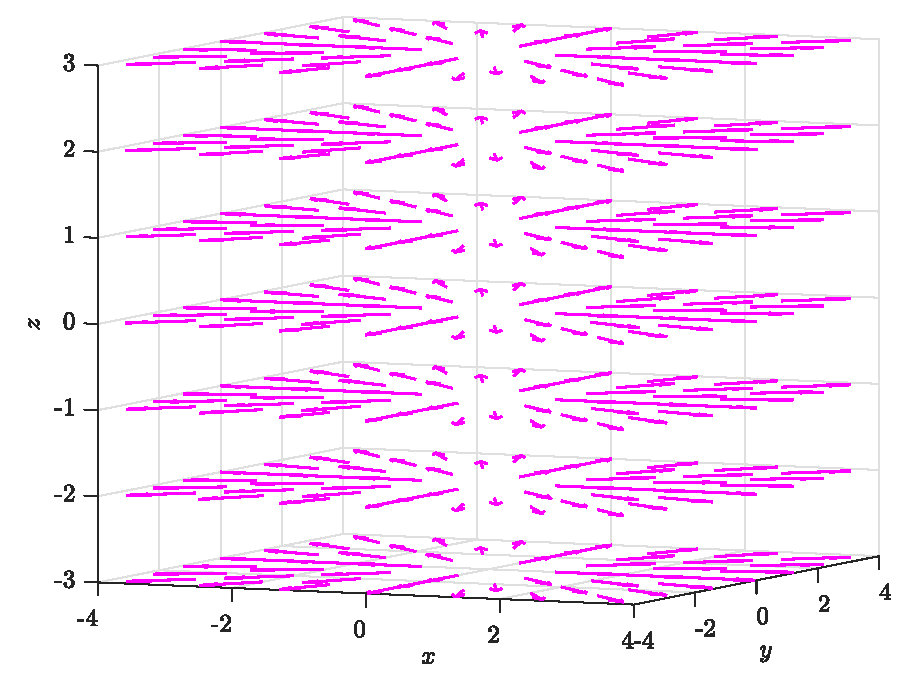
\includegraphics[width=.6\textwidth]{figures/rho_hat}
    \end{figure}
    Notice that when $x=y=0$ (i.e., along the $z$-axis) that we have an inability to ascribe a direction to $\rhohat$. This is because the coordinate $\rho$ itself is defined to be the measurement of distance from the $z$-axis. The field $\rhohat$ points in the direction in which $\rho$ increases most quickly (i.e., it points along $\grad \rho(x,y,z)$). Since any direction satisfies this idea, there is no unique direction to choose. This vector field is unable to describe anything useful along the $z$-axis.

    \item Here is a plot of $\thetahat$.
    \begin{figure}[H]
        \centering
        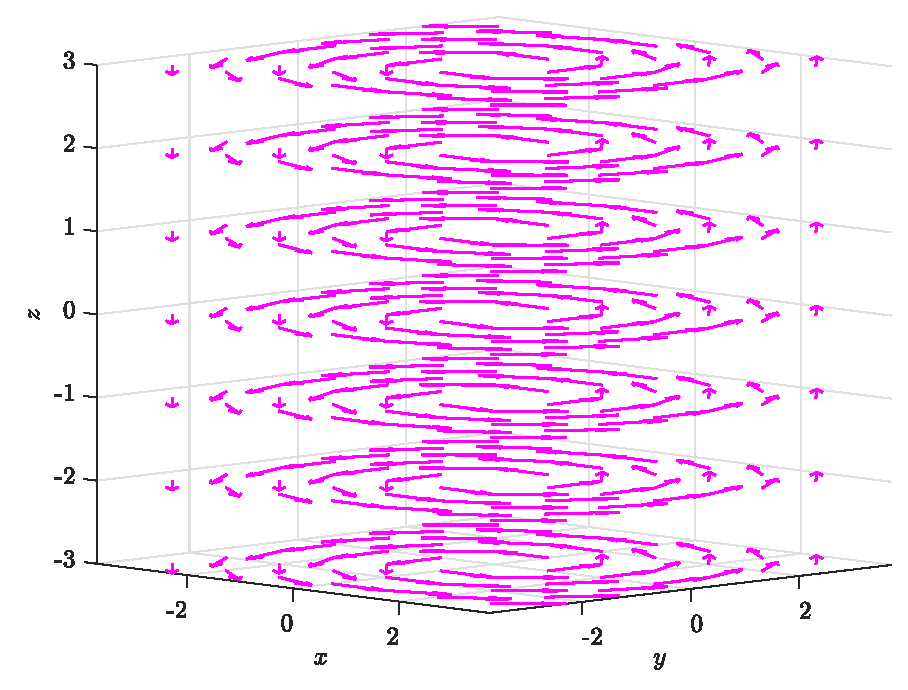
\includegraphics[width=.6\textwidth]{figures/theta_hat}
    \end{figure}
    Much like $\rhohat$, $\thetahat$ has issues along the $z$-axis. But, the reason for issue is subtly different than the failure of $\rhohat$. If we pick a point with $x\neq 0$ or $y\neq 0$, then we can ascribe an angle to this vector relative to the $xz$-plane. However, for points on the $z$-axis, there is no angle to speak of -- it isn't that it is a zero angle, it simply does not exist. 

    \item Here is a plot of $\phihat$.
    \begin{figure}[H]
        \centering
        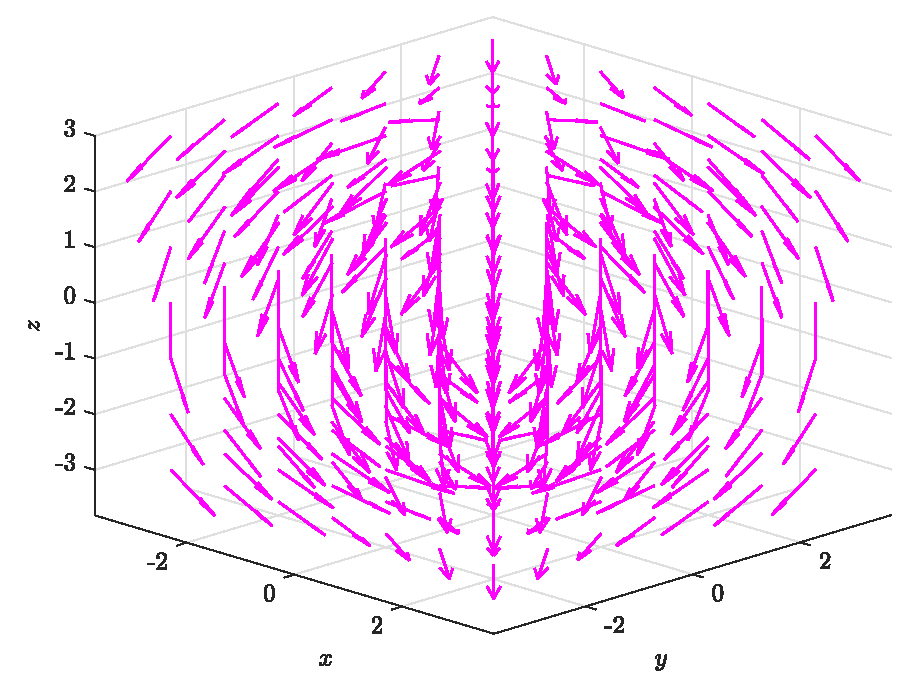
\includegraphics[width=.6\textwidth]{figures/phi_hat}
    \end{figure}
    This vector field again lacks a description along the $z$-axis since we would have $x=y=0$. Once again, the reasoning here is subtle yet important. A point on the $z$-axis either has an angle of $\phi = 0$ or $\phi = \pi$ and, for the origin, there isn't a valid angle to specify there either. Once again, we can think about what direction moving away from the $z$-axis would increase $\phi$ (i.e., point in $\phihat$), and the answer is \emph{every} direction does this. 

    \item Here is a plot of $\rhat$.
    \begin{figure}[H]
        \centering
        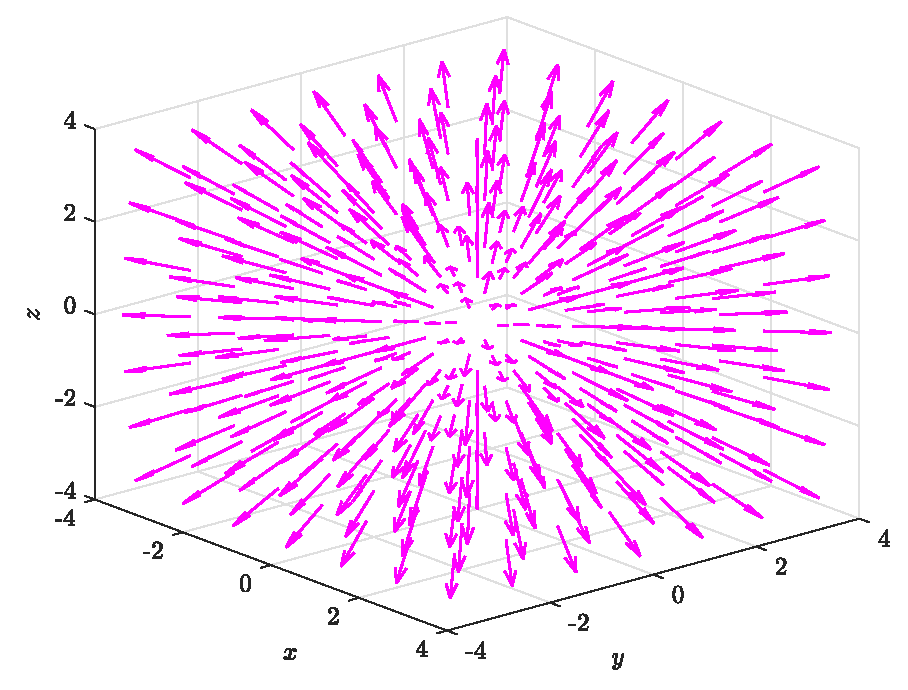
\includegraphics[width=.6\textwidth]{figures/r_hat}
    \end{figure}
    This field experiences only a single point of concern. Namely, the origin. There, this field is not defined as any direction we choose to move at the origin increases $r$ since $r$ is a measure of distance from the origin. 
\end{enumerate}
\end{solution}
\vspace*{1cm}
\textcolor{red}{
\noindent \textbf{Rubric:}
\begin{enumerate}[(a)]
    \item \textbf{(1 pt.)} Correct \textbf{AND} interpretable plot. \textbf{(1 pt.)} Reasonable explanation for what each field represents and some mention of where the field fails to provide a coordinate.
    \item \textbf{(1 pt.)} Correct \textbf{AND} interpretable plot. \textbf{(1 pt.)} Reasonable explanation for what each field represents and some mention of where the field fails to provide a coordinate.
    \item \textbf{(1 pt.)} Correct \textbf{AND} interpretable plot. \textbf{(1 pt.)} Reasonable explanation for what each field represents and some mention of where the field fails to provide a coordinate.
    \item \textbf{(1 pt.)} Correct \textbf{AND} interpretable plot. \textbf{(1 pt.)} Reasonable explanation for what each field represents and some mention of where the field fails to provide a coordinate.
\end{enumerate}
}

\newpage
\begin{problem}
	\textbf{(14 pts.)} Let us see some of the usefulness of cylindrical coordinates.
	\begin{enumerate}[(a)]
		\item \textbf{(1 pts.)} Using the fact that $\thetahat = \frac{-y}{\sqrt{x^2+y^2}}\xhat + \frac{x}{\sqrt{x^2+y^2}}\yhat$, convert the magnetic field 
		\[
		\vecfieldB = -\frac{y}{2}\xhat + \frac{x}{2}\yhat,
		\]
		into cylindrical coordinates (i.e., only a function of $\rho$, $\theta$, $z$, and $\rhohat$, $\thetahat$, and $\zhat$).  
		\item \textbf{(2 pts.)} Parameterize a curve $\curvegamma(t)$ that traces out a circle of radius $R$ in the $xy$-plane in cylindrical coordinates.
		\item \textbf{(2 pts.)} Compute the velocity vector $\tangentgamma(t)$ in cylindrical coordinates.
		\item \textbf{(2 pts.)} Compute the acceleration vector $\normalgamma(t)$ in cylindrical coordinates.
		\item \textbf{(3 pts.)} Compute the following integral using cylindrical coordinates
		\[
		\int_{\curvegamma} \vecfieldB \cdot d\curvegamma.
		\]
		        \item \textbf{(4 pts.)} Using cylindrical coordinates, compare your result with
		        \[
		        \iint_\Sigma \left(\grad \times \vecfieldB\right) \cdot \unitvec d\Sigma,
		        \]
		        where $\Sigma$ is the disk of radius $R$. In other words, the surface that fills in the curve from before.
	\end{enumerate}
\end{problem}
\begin{solution}~
\begin{enumerate}[(a)]
    \item We have that
    \[
    \vecfieldB = -\frac{y}{2} \xhat + \frac{x}{2}\yhat.
    \]
    Then, note that we have
    \begin{align*}
        \vecfieldB &= \frac{1}{2}\sqrt{x^2+y^2} \left( \frac{-y}{\sqrt{x^2+y^2}} \xhat + \frac{x}{\sqrt{x^2+y^2}} \right)\\
        &=\frac{1}{2} \sqrt{x^2+y^2} \thetahat.
    \end{align*}
    Finally, we have that $\rho = \sqrt{x^2+y^2}$ and hence
    \[
    \vecfieldB = \frac{\rho}{2} \thetahat.
    \]

    \item It suffices to find functions $\rho(t)$, $\theta(t)$, and $z(t)$ to create the curve
    \[
    \curvegamma(t) = \rho(t) \rhohat + \theta(t) \thetahat + z(t) \zhat.
    \]
    Note that for a circle of radius $R$ centered along the $z$-axis, we have that $\rho=R$ is constant.  Similarly, we want the circle to lie in the $xy$-plane where $z=0$, hence we must have $z(t)=0$.  Finally, we must trace the whole unit circle so we must have $\theta$ cover all of $[0,2\pi)$. One choice is to have $\theta(t)=t$ for $t\in[0,2\pi)$, but there are many other options! Using these choices, we have
    \[
    \curvegamma(t) = \rhohat + t \thetahat.
    \]
    \item Then, we have the tangent vector $\tangentgamma = \dot{\rho}\rhohat + \rho \dot{\theta} \thetahat + z \zhat$ and thus
    \[
    \boxed{\tangentgamma(t) = R \thetahat.}
    \]

	\item The acceleration vector is given by
	\[
	\normalgamma(t) = (\ddot{\rho}+\rho \dot{\theta}^2) \rhohat + (2 \dot{\rho} \dot{\theta}+\rho \ddot{\theta}^2)\thetahat + \ddot{z}\zhat
	\]
	so in our case we have
	\[
	\boxed{\normalgamma(t)= R \rhohat.}
	\]

    \item Note that from the above work we have
    \[
    d \curvegamma = \tangentgamma dt = R \thetahat dt.
    \]
    Thus, 
    \[
    \vecfieldB(\gamma(t)) \cdot \tangentgamma = \frac{\rho(\gamma(t)) R}{2} = \frac{R^2}{2}
    \]
    This gives us that
    \begin{align*}
        \int_{\curvegamma} \vecfieldB \cdot d\curvegamma &= \int_0^{2\pi} \frac{R^2}{2}dt\\
        &= \pi R^2.
    \end{align*}
    It should actually not be all that surprising that this ends up being the area of a disk of radius $R$!

	\item We have computed the curl of this field before, but it is
	\[
\grad \times \vecfieldB = \zhat.
	\]
Similarly, the normal vector to the disk of radius $R$ in the $xy$-plane is $\unitvec = \zhat$ (up to choice of orientation that is). Hence, we have
\begin{align*}
	\iint_{\Sigma} (\grad \times \vecfieldB) \cdot \unitvec d \Sigma  &= \int_0^{2\pi } \int_{0}^R \rho d \rho d \theta\\
	&= \pi R^2.
\end{align*}
Once again, we get the area of a disk of radius $R$.
\end{enumerate}
\end{solution}
\vspace*{1cm}
\textcolor{red}{
\noindent \textbf{Rubric:}
\begin{enumerate}[(a)]
    \item \textbf{(1 pt.)} Correct conversion. 
    \item \textbf{(1 pt.)} Correct parameterization with start and end points. \textbf{(1 pt.)} Arbitrary $R$ used. No specific value of $R$!
    \item \textbf{(1 pt.)} Given in terms of correct coordinates. \textbf{(1 pt.)} Correct velocity vector.
    \item \textbf{(1 pt.)} Given in terms of correct coordinates. \textbf{(1 pt.)} Correct acceleration vector.
	\item \textbf{(1 pt.)} Correct $d \curvegamma$. \textbf{(1 pt.)} Correct $\vecfieldB(\curvegamma(t))$ and dot product. \textbf{(1 pt.)} Correct value for integral including arbitrary $R$.
	\item \textbf{(1 pt.)} Correct $d \Sigma$. \textbf{(1 pt.)} Correct $\grad \times \vecfieldB$, normal vector $\unitvec$, and dot product. \textbf{(1 pt.)} Correct value for integral including arbitrary $R$. \textbf{(1 pt.)} Relate it back to the curve integral.
\end{enumerate}
}

\newpage
\begin{problem}
	\textbf{(4 pts.)} Convert the following integrals to integrals in cylindrical coordinates. Also, describe the region in which you are integrating over. Do not evaluate the integrals.
	\begin{enumerate}[(a)]
		\item \textbf{(2 pts.)} $\displaystyle{\int_{-1}^{1} \int_{-1}^{1} \int_{-\sqrt{1-y^2}}^{\sqrt{1-y^2}} xyz dxdydz}$.
		\item \textbf{(2 pts.)} $\displaystyle{\int_0^1 \int_{-z}^z \int_{-\sqrt{z^2-y^2}}^{\sqrt{z^2-y^2}} x^2+y^2+z^2 dxdydz}$.
	\end{enumerate}
\end{problem}
\begin{solution}~
\begin{enumerate}[(a)]
    \item First, let us convert the integrand to cylindrical coordinates. We have
    \[
    xyz = \rho \cos (\theta) \rho \sin(\theta) z = \rho^2 \cos(\theta)\sin(\theta)z.
    \]
    Now, as for the bounds to the integral, we are letting
    \[
    -\sqrt{1-y^2}\leq x \leq \sqrt{1-y^2}.
    \]
    In other words, this is the region given in the following figure.
    \begin{figure}[H]
        \centering    
    \includegraphics[width=.6\textwidth]{figures/disk.png}
    \end{figure} 
    So, if we then let $y$ range from $-1$ to $1$, we must be integrating over the unit disk in the $xy$-plane.  Then, we have $-1\leq z\leq 1$, so it must be that we are integrating over a cylindrical region.  So, to convert the whole integral to cylindrical coordinates, we note that
    \[
    dxdydz = \rho d\rho d\theta dz,
    \]
    and thus
    \[
    \int_{-1}^{1} \int_{-1}^{1} \int_{-\sqrt{1-y^2}}^{\sqrt{1-y^2}} xyz dxdydz = \int_{-1}^1 \int_{0}^{2\pi} \int_{0}^1 \rho^3 \cos(\theta)\sin(\theta)z d\rho d\theta dz.
    \]
    \item The intuition from (a) can help us since the bounds for $x$ and $y$ are similar to (a), except that we have that the radius of the circle depends is equal to $z$ and is not just fixed at 1. In other words, as $z$ increases, we are integrating over larger disks. The disks increase from a radius of 0 up to a radius of 1 linearly, so we are integrating over a solid cone!

    In fact, one way to see this is to mess with the above equations
    \begin{align*}
        -\sqrt{z^2-y^2}\leq &x \leq \sqrt{z^2-y^2} \\
        \implies ~ x^2&= z^2-y^2 \\
        \implies ~ x^2+y^2-z^2=0,
    \end{align*}
    which is the implicit equation for a double cone surface. In cylindrical coordinates, this gives us the relationship $\rho^2=z^2$ and thus $z=\pm\rho$. However, we require $0\leq z \leq 1$, so we must take $\rho=z$.  Thus, our integral then becomes
    \[
    \int_0^1 \int_{-z}^z \int_{-\sqrt{z^2-y^2}}^{\sqrt{z^2-y^2}} x^2+y^2+z^2 dx\,dy\,dz = \int_{0}^1 \int_0^{2\pi} \int_{0}^z \left(\rho^2 + z^2 \right) \rho \, d\rho \, d \theta\, dz. 
    \]
    \end{enumerate}
\end{solution}
\vspace*{1cm}
\textcolor{red}{
\noindent \textbf{Rubric:}
\begin{enumerate}[(a)]
    \item \textbf{(1 pt.)} Correct conversion including $\rho d\rho d \theta dz$. \textbf{(1 pt.)} Correct description of region of integration.
	\item \textbf{(1 pt.)} Correct conversion including $\rho d\rho d \theta dz$. \textbf{(1 pt.)} Correct description of region of integration.
\end{enumerate}
}

\newpage
\begin{problem}
	\textbf{(2 pts.)} Note that the Laplacian $\Delta$ in cylindrical coordinates is given by
	\[
	\Delta f(\rho,\theta,z) = \frac{1}{\rho} \frac{\partial}{\partial \rho} \left(\rho \frac{\partial f}{\partial \rho}\right)+\frac{1}{\rho^2}\frac{\partial^2 f}{\partial \theta^2} + \frac{\partial^2 f}{\partial z^2}.
	\]
	Compute the Laplacian of
	\[
	f(\rho,\theta,z) = \sqrt{\rho^2+z^2} z \cos(\theta).
	\]
\end{problem}
\begin{solution}
Let's compute each term and then add them together. We have
\begin{align*}
    A=\frac{1}{\rho}\frac{\partial}{\partial \rho} \left(\rho \frac{\partial f}{\partial \rho} \right) &=  \frac{z\cos \theta}{\rho} \frac{\partial}{\partial \rho} \left( \frac{\rho^2}{\sqrt{\rho^2+z^2}} \right)\\
    &=\frac{z\cos \theta}{\rho} \left(\frac{2\rho}{\sqrt{\rho^2+z^2}}-\frac{\rho^3}{\rho^2+z^2}\right)\\
    &= z\cos \theta \left( \frac{2}{\sqrt{\rho^2+z^2}} - \frac{\rho^2}{\left(\rho^2+z^2\right)}\right).
\end{align*}
Likewise, we have
\begin{align*}
    B=\frac{1}{\rho^2} \frac{\partial^2 f}{\partial \theta^2} &= -\frac{\sqrt{\rho^2+z^2}z\cos\theta}{\rho^2}.
\end{align*}  
Lastly, we have
\begin{align*}
    C=\frac{\partial^2 f}{\partial z^2} &= \cos \theta \frac{\partial}{\partial z}\frac{\partial}{\partial z} \left( z \sqrt{\rho^2+z^2}\right)\\
    &= \cos \theta \frac{\partial}{\partial z} \left( \sqrt{\rho^2+z^2}+ \frac{z^2}{\sqrt{\rho^2+z^2}}\right)\\
    &= \cos \theta \left(\frac{z}{\sqrt{\rho^2+z^2}}+\frac{2z}{\sqrt{\rho^2+z^2}}-\frac{z^3}{\left(\rho^2+z^2\right)^{3/2}}\right).
\end{align*}
Then we have that
\[
\Delta f = A+B+C.
\]
\end{solution}
\vspace*{1cm}
\textcolor{red}{
\noindent \textbf{Rubric:}
\begin{enumerate}[(a)]
    \item \textbf{(1 pt.)} Correct derivatives including work or WolframAlpha. \textbf{(1 pt.)} Correct final answer for Laplacian.
\end{enumerate}
}

\newpage
\begin{problem}
	\textbf{(8 pts.)} In spherical coordinates (either implicitly or explicitly), parameterize the following objects.
	\begin{enumerate}[(a)]
		\item \textbf{(2 pts.)} A solid sphere with radius 3.
		\item \textbf{(2 pts.)} The surface of an infinite cone with a vertex angle of $\pi/4$.
		\item \textbf{(2 pts.)} A latitudinal curve on the unit sphere at the latitude of 30$^\circ$ above the equator.
		\item \textbf{(2 pts.)} A solid unit sphere with a cylinder of radius 1/2 removed from the core.
	\end{enumerate}
\end{problem}
\begin{solution} ~
 \begin{enumerate}[(a)]
    \item In this case, it's easiest to just take $0\leq r \leq 3$, $0\leq \theta < 2\pi$ and $0\leq \phi \leq \pi$.  
    \item Here, we let $\phi=\frac{\pi}{8}$ so that the vertex angle is $\frac{\pi}{4}$.  Then we let $r\in [0,\infty)$ and $\theta \in [0,2\pi)$.
    \item We can write this in spherical coordinates by noting that 30$^\circ$ is $\frac{\pi}{6}$ and that we can get $\phi(t)$ must be constant and indeed 
    \[
    \phi(t) = \frac{\pi}{2}-\frac{\pi}{6}=\frac{\pi}{3}.
    \]
    Then, since the curve is on the unit sphere, it must be that $r(t)=1$ and finally we have freedom to choose $\theta(t)$ so long as $\theta$ runs over the range $[0,2\pi)$. Most easily is to take $\theta(t)=t$ and $t\in [0,2\pi)$ to get the curve
    \[
    \curvegamma(t) = \rhat + t \thetahat +\frac{\pi}{3} \phihat.
    \]
    \item Recall that a cylinder of radius $\frac{1}{2}$ has the equation
    \[
    x^2+y^2=\frac{1}{4}.
    \]
    The unit sphere is given by $r\leq 1$ with $\theta \in [0,2\pi)$ and $\phi \in [0,\pi]$. However, one can see that for this object to be properly parameterized, we need that $r$ depends on $\phi$.  Drawing from a side profile can lead one to find that we must always have the small value for $r$ is
    \[
    r_{\textrm{min}} \sin \phi = \frac{1}{2}
    \]
    Then, it must be that at smallest $\phi = \frac{\pi}{6}$ since when $r=1$ we have $\phi = \arcsin(1/2) = \frac{\pi}{6}$.  So, the description is given by $\phi \in [\pi/6, 5\pi/6]$ with $\frac{1}{2\sin \phi} \leq r \leq 1$ and $\theta \in [0,2\pi)$.
 \end{enumerate}
\end{solution}
\vspace*{1cm}
\textcolor{red}{
\noindent \textbf{Rubric:}
\begin{enumerate}[(a)]
    \item \textbf{(1 pt.)} Parameterization is a solid. \textbf{(1 pt.)} Correct parameterization in spherical coordinates.
\item \textbf{(1 pt.)} Parameterization is a surface. \textbf{(1 pt.)} Correct parameterization in spherical coordinates.
\item \textbf{(1 pt.)} Parameterization is a curve. \textbf{(1 pt.)} Correct parameterization in spherical coordinates.
\item \textbf{(1 pt.)} Parameterization is a solid. \textbf{(1 pt.)} Correct parameterization in spherical coordinates.
\end{enumerate}
}

\newpage
\begin{problem}
	\textbf{(8 pts.)} Let us see some of the benefit of using spherical coordinates. 
	\begin{enumerate}[(a)]
		\item \textbf{(1 pts.)} Using the fact that 
		\[
		\rhat = \frac{x}{\sqrt{x^2+y^2+z^2}}\xhat + \frac{y}{\sqrt{x^2+y^2+z^2}}\yhat + \frac{z}{\sqrt{x^2+y^2+z^2}}\zhat,
		\]
		convert the vector field 
		\[
		\vecfieldE(x,y,z) = \begin{pmatrix} \frac{x}{(x^2+y^2+z^2)^{3/2}} \\ \frac{y}{(x^2+y^2+z^2)^{3/2}} \\ \frac{z}{(x^2+y^2+z^2)^{3/2}} \end{pmatrix},
		\] into spherical coordinates (i.e., only a function of $r$, $\theta$, $\phi$, and $\rhat$, $\thetahat$, and $\phihat$).
		\item \textbf{(2 pts.)} Parameterize the surface of a sphere of radius $R$ (which we'll call $\Sigma$) as well as the outward normal vector $\unitvec$ and  in spherical coordinates.
		\item \textbf{(3 pts.)} Compute the following integral using spherical coordinates that we have found:
		\[
		\iint_\Sigma \vecfieldE \cdot \unitvec d\Sigma,
		\]
		where $d\Sigma$ will be the area form in spherical coordinates.
		\item \textbf{(2 pts.)} You computed a similar integral in an earlier problem on this homework. Does the total flux depend on the size or shape of the surface enclosing the origin? Explain.
	\end{enumerate}
\end{problem}
\begin{solution}~
\begin{enumerate}[(a)]
    \item We have
    \begin{align*}
    \vecfieldE &= \frac{x}{\left(x^2+y^2+z^2\right)^{3/2}} \xhat + \frac{y}{\left(x^2+y^2+z^2\right)^{3/2}} \yhat + \frac{z}{\left(x^2+y^2+z^2\right)^{3/2}} \zhat\\
     &= \frac{1}{x^2+y^2+z^2} \left( \frac{x}{\sqrt{x^2+y^2+z^2}} \xhat + \frac{y}{\sqrt{x^2+y^2+z^2}} \yhat + \frac{z}{\sqrt{x^2+y^2+z^2}} \zhat\right)\\
     &= \frac{1}{x^2+y^2+z^2} \rhat\\
     &= \frac{1}{r^2} \rhat.
    \end{align*}
    \item We have the parameterization of the surface of a unit sphere given by letting $r=R$ and $\theta \in [0,2\pi)$ and $\phi \in [0,\pi]$. We can use the implicit equation $f(r,\theta,\phi)=r-R$ to find the surface normal by
    \begin{align*}
        \unitvec &= \frac{\grad f}{\left| \grad f \right|} \\
        &= \frac{\grad r}{\left|\grad r\right|}\\
        &= \rhat,
    \end{align*}
    by definition. This was done in a previous homework in cartesian coordinates as well.
    \item From the previous work, we have that
    \[
    \vecfieldE \cdot \unitvec = \frac{1}{r^2}.  
    \]
    Then, this gives us
    \begin{align*}
        \iint_{\Sigma} \vecfieldE \cdot \unitvec d\Sigma &= \int_0^\pi \int_0^{2\pi} \frac{1}{R^2} R^2 \sin \phi  \, d\theta \, d\phi \\
        &= 2\pi \int_0^\pi \sin \phi \, d \phi\\
        &= 4 \pi.  
    \end{align*}
    One can notice that the radius of the sphere (so long as it is nonzero) does not come into play here. 
\item No, we have found in this problem that the radius of the sphere does not change the integral. We also got the same value of the integral when we integrated over the surface of a cubic box. It seems as if the shape and size of the surface doesn't matter; really all that matters is it encloses the origin where the ``charge" is located. This is Gauss's law!
\end{enumerate} 
\end{solution}
\vspace*{1cm}
\textcolor{red}{
\noindent \textbf{Rubric:}
\begin{enumerate}[(a)]
    \item \textbf{(1 pt.)} Correct conversion.
\item \textbf{(1 pt.)} Correct parameterization in spherical coordinates. \textbf{(1 pt.)} Correct normal vector.
\item \textbf{(1 pt.)} Correct $\vecfieldE \cdot \unitvec$ \textbf{(1 pt.)} Correct bounds for integral. \textbf{(1 pt.)} Correct value for integral.
\item \textbf{(1 pt.)} Realize that the size of the sphere does not matter in this problem. \textbf{(1 pt.)} Realize that both the box and sphere had the same answer, so the shape seems to not matter.
\end{enumerate}
}

\newpage
\begin{problem}
    Note that the Laplacian $\Delta$ in spherical coordinates is given by
    \[
        \Delta f(r,\theta,\phi) = \frac{1}{r^2} \frac{\partial}{\partial r} \left(r^2 \frac{\partial f}{\partial r}\right)+\frac{1}{r^2 \sin^2 \phi} \frac{\partial^2 f}{\partial \theta^2} + \frac{1}{r^2 \sin\phi}\frac{\partial}{\partial \phi} \left(\sin \phi \frac{\partial f}{\partial \phi}\right).
    \]
    Compute the Laplacian of
    \[
       f(r,\theta,\phi) = r^2 \cos(\theta)\cos(\phi).
    \]
\end{problem}
\begin{solution}
 Again, we will do this piece by piece. First, we have
 \begin{align*}
    A=\frac{1}{r^2}\frac{\partial}{\partial r} \left(r^2 \frac{\partial f}{\partial r}\right)&= \frac{\cos (\theta) \cos (\phi)}{r^2}\frac{\partial}{\partial r} \left(2r^3\right) \\
    &= \frac{\cos (\theta) \cos(\phi)}{r^2} 6r^2\\
    &= 6 \cos (\theta) \cos (\phi).
 \end{align*}
 Next, we have
 \begin{align*}
    B=\frac{1}{r^2 \sin \phi} \frac{\partial^2 f}{\partial \theta^2} &= \frac{1}{r^2 \sin \phi} (-r^2\cos(\theta)\cos(\phi))\\
    &= -\frac{\cos(\theta)\cos(\phi)}{\sin\phi}
 \end{align*}
 Lastly, we have
 \begin{align*}
    C=\frac{1}{r^2\sin \phi} \frac{\partial }{\partial \phi} \left(\sin \phi \frac{\partial f}{\partial \phi}\right)&= \frac{1}{r^2\sin \phi} \frac{\partial }{\partial \phi} \left( -r^2 \cos(\theta) \sin^2(\phi)\right)\\
&=\frac{1}{r^2 \sin \phi} -2r^2 \cos(\theta)\sin(\phi)\cos(\phi)\\
&=-2\cos(\theta)\cos(\phi).
 \end{align*}
 Then,
 \[
 \Delta f = A+B+C.
 \]
\end{solution}
\vspace*{1cm}
\textcolor{red}{
\noindent \textbf{Rubric:}
\begin{enumerate}[(a)]
    \item \textbf{(1 pt.)} Correct derivatives including work or WolframAlpha. \textbf{(1 pt.)} Correct final answer for Laplacian.
\end{enumerate}
}

\end{document}